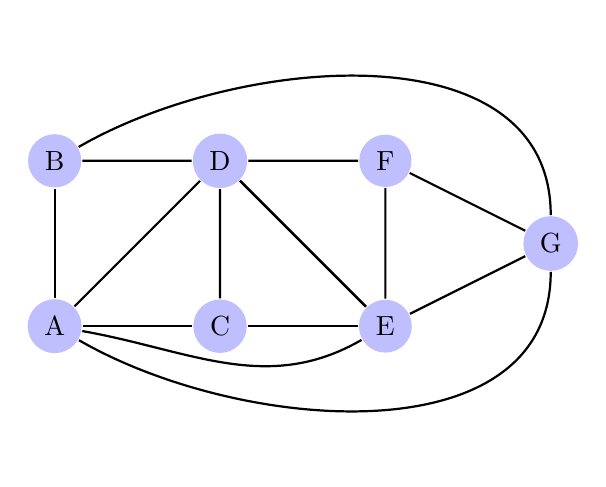
\begin{tikzpicture}
[thick,scale=.7,auto=left,every node/.style={circle,fill=blue!25}]
  \node (n6) at (3,2) {A};
  \node (n4) at (3,5) {B};
  \node (n5) at (6,2) {C};
  \node (n1) at (6,5) {D};
  \node (n2) at (9,2) {E};
  \node (n3) at (9,5) {F};
  \node (n7) at (12,3.5) {G};
  \foreach \from/\to in {n6/n4,n5/n1,n2/n3,n4/n1,n6/n1,n1/n2,n3/n7,n7/n2,n5/n6,n5/n2,n1/n2,n1/n3}
    \draw (\from) -- (\to);
    \draw (n4) to[out=30,in=90] (n7);
    \draw (n6) to[out=-10,in=-150] (n2);
    \draw (n6) to[out=-30,in=-90] (n7);
\end{tikzpicture}